\subsection{Visualisierungsmöglichkeiten und Zielgruppe}
\label{sub:visualisierungsmöglichkeiten_und_zielgruppe}

  Das gesammelte Material zu den möglichen Visualisierungsarten wurde in einer 2x2 Matrix (Abbildung \ref{fig:2x2_matrix}) in die Unterkategorien "`Live Map, Künstlerische Visualisierung, Plugin / Software / Tool, Tube-Map"' eingeordnet, um einen sortierten Gesamtüberblick zu bekommen. 

  \begin{figure}[htbp]
    \begin{center}
      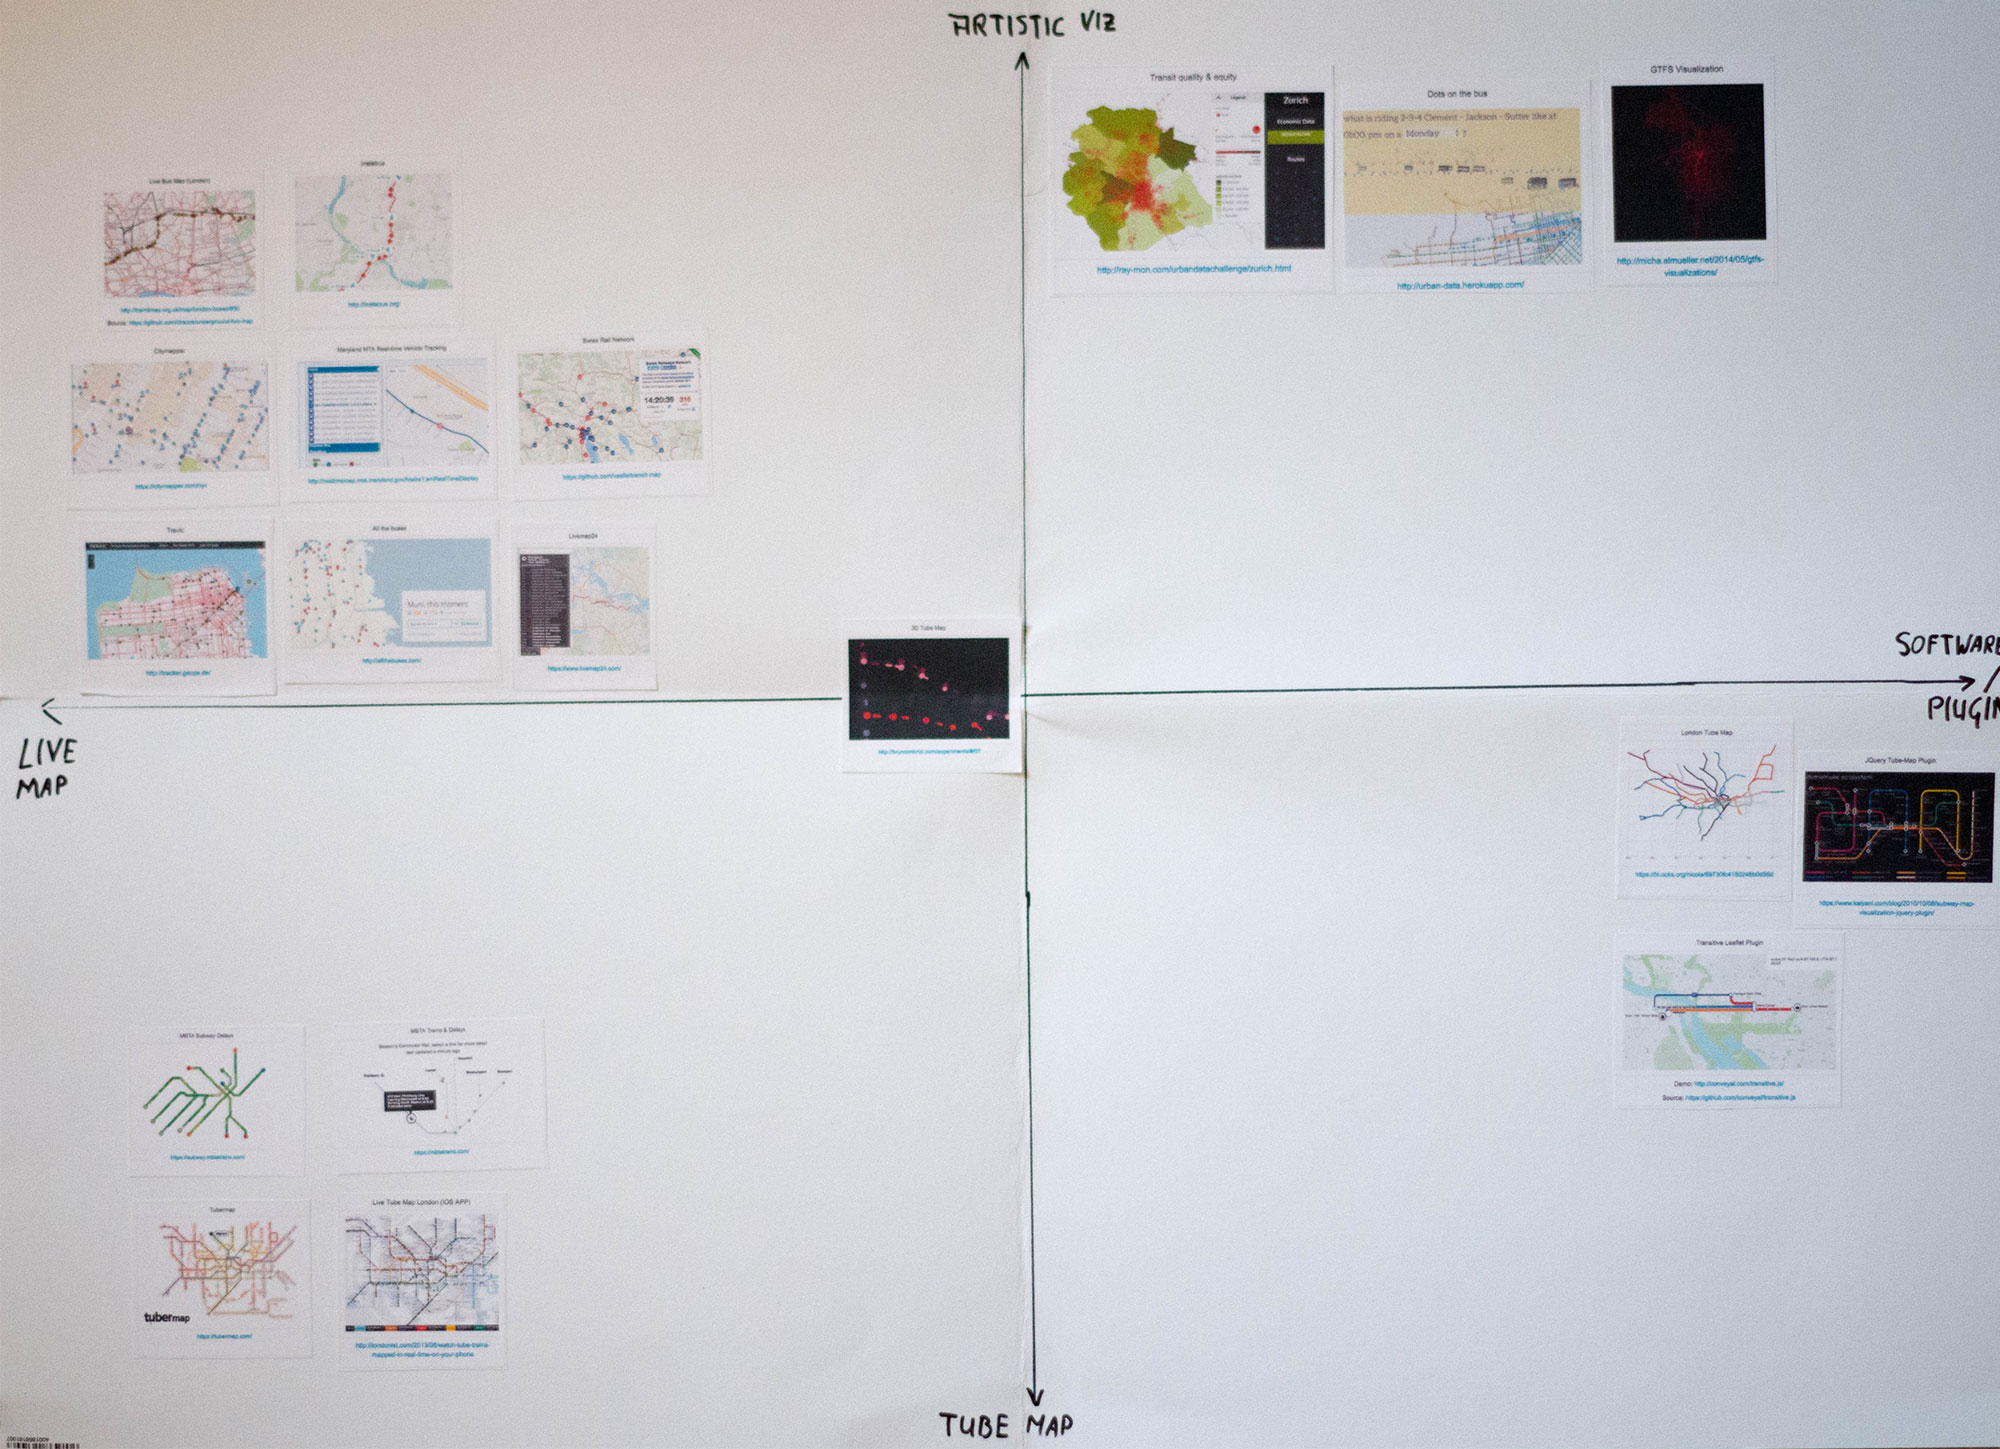
\includegraphics[width=0.5\textwidth]{2x2_matrix}
      \caption{2x2 Matrik Methode auf DIN A2}
      \label{fig:2x2_matrix}
    \end{center}
  \end{figure}

  Durch diese Ansicht wurde die Erkenntnis gewonnen, dass es schon viele Live Visualisierungen auf interaktiven Karten gibt, aber nur sehr wenig so genannte Tube-Maps. Auch sind bereits verschiedenste Tools zum Generieren von GTFS-basierten Visualisierungen vorhanden. Eine sehr ausführliche, aber bei weitem nicht vollständige Liste über das Thema "`Transit"' wurde auf Github von der Community zusammengetragen \url{https://github.com/luqmaan/awesome-transit}.

  % TODO: Eventuell Personas?

% subsection visualisierungsmöglichkeiten_und_zielgruppe (end)